\documentclass{beamer}

%\usetheme[hideothersubsections]{UNLTheme}
\beamertemplatenavigationsymbolsempty

\mode<presentation> {
    \usetheme[hideothersubsections]{UNLTheme}
    %\usetheme{montpellier}
    \setbeamercovered{transparent}
}

\usepackage[cp1250]{inputenc}
\usepackage[IL2]{fontenc}
\usepackage[english]{babel}
\usepackage{color}
\usepackage{multimedia}
\usepackage{amsbsy}
\usepackage{amsfonts}
\usepackage{amssymb}
\usepackage{mathrsfs}
\usepackage{enumerate}
\usepackage{amsthm}
%\usepackage{showkeys}
\usepackage{gensymb}
\usepackage{amsmath} % balíček pro pokročilou matem. sazbu
\usepackage{epsfig} % balíčky pro vkládání grafických souborů typu EPS
\usepackage{graphicx}
\usepackage{listings}

\definecolor{dkgreen}{rgb}{0,0.6,0}
\definecolor{gray}{rgb}{0.5,0.5,0.5}
\definecolor{mauve}{rgb}{0.58,0,0.82}

\lstset{frame=tb,
    language=Python,
    aboveskip=3mm,
    belowskip=3mm,
    showstringspaces=false,
    columns=flexible,
    basicstyle={\small\ttfamily},
    numbers=none,
    numberstyle=\tiny\color{gray},
    keywordstyle=\color{blue},
    commentstyle=\color{dkgreen},
    stringstyle=\color{mauve},
    breaklines=true,
    breakatwhitespace=true,
    tabsize=3
}

\newcommand{\e}{\mathtt{e}}
\newcommand{\R}{\mathbf{R}}
\newcommand{\N}{\mathbf{N}}
\newcommand{\Z}{\mathbf{Z}}
\newcommand{\proceseta}{\boldsymbol{\eta}}
\newcommand{\dr}{\, \mathrm{d}}
\newtheorem{veta}{Theorem}[section]
\newtheorem{defin}[veta]{Definition}


\title{Encoding Of Categorical Variables}
\author{Michael Mat\v{e}j\r{u}}
\institute[KB]{AI Squad}
\date{\today}

\begin{document}

    \begin{frame}
        \titlepage
    \end{frame}

    \begin{frame}
        \frametitle{Outline}
        \tableofcontents
    \end{frame}


    \section{Motivation}
    \begin{frame}
        \frametitle{Motivation}
        \begin{itemize}
            \item MRMR Feature Selection Algorithm implemented by Smazzanti
            \pause
            \item For categorical encoding he used three target based algorithms
            \pause
            \item And inspite of all common sense it works in Kaggle Challanges
            \pause
            \item There is no free lunch.
            \pause
            \item Regularization is a must for target-based encoders.
        \end{itemize}
    \end{frame}


    \section{Toy Dataset}
    \begin{frame}
        \frametitle{Toy Dataset}
        \begin{table}[htb]
            \begin{center}
            {\renewcommand{\arraystretch}{0.4}
            \renewcommand{\tabcolsep}{0.4cm}
                \begin{tabular}[c]{|c|c|c|}
                    \hline & \textbf{category} & \textbf{target} \\
                    \hline
                    0      & A                 & 0               \\
                    \hline
                    1      & A                 & 1               \\
                    \hline
                    2      & A                 & 0               \\
                    \hline
                    3      & A                 & 1               \\
                    \hline
                    4      & B                 & 0               \\
                    \hline
                    5      & B                 & 1               \\
                    \hline
                    6      & B                 & 0               \\
                    \hline
                    7      & C                 & 1               \\
                    \hline
                    8      & C                 & 0               \\
                    \hline
                    9      & D                 & 1               \\
                    \hline
                \end{tabular}}
                \caption{Toy Dataset}
            \end{center}
        \end{table}
    \end{frame}


    \section{Categorical Encoders}
    \begin{frame}
        \frametitle{Types}
        \begin{itemize}
            \item Target-Based Encoders
            \item The Rest
        \end{itemize}
    \end{frame}

    \subsection{Non-Target Based Encoders}
    \begin{frame}[fragile]
        \frametitle{Label / Ordinary Encoder}
        \begin{itemize}
            \item One of the most common algorithms
            \item Encodes into N integers
            \pause
        \end{itemize}

        \begin{lstlisting}
LE_encoder = OrdinalEncoder(feature_list)
train_le = LE_encoder.fit_transform(train)
test_le = LE_encoder.transform(test)
        \end{lstlisting}
    \end{frame}

    \begin{frame}[fragile]
        \frametitle{One Hot Encoder}
        \begin{itemize}
            \item One of the most common algorithms
            \item Encodes columns with N categories into N-1 boolean columns
            \pause
        \end{itemize}

        \begin{lstlisting}
traintest = pd.concat([train, test])
dummies = pd.get_dummies(traintest, columns=traintest.columns, drop_first=True, sparse=True)
train_ohe = dummies.iloc[:train.shape[0], :]
test_ohe = dummies.iloc[train.shape[0]:, :]
train_ohe = train_ohe.sparse.to_coo().tocsr()
test_ohe = test_ohe.sparse.to_coo().tocsr()
        \end{lstlisting}
    \end{frame}

    \begin{frame}[fragile]
        \frametitle{Sum / Deviation Encoder}
        \begin{itemize}
            \item Similar to One Hot Encoder
            \item Difference is in interpretation of LR coefficients.
            \pause
        \end{itemize}

        \begin{lstlisting}
# this method didn't work because of low RAM memory.
# SE_encoder =SumEncoder(feature_list)
# train_se = SE_encoder.fit_transform(train[feature_list], target)
# test_se = SE_encoder.transform(test[feature_list])
        \end{lstlisting}
    \end{frame}

    \begin{frame}[fragile]
        \frametitle{Helmert Encoder}
        \begin{itemize}
            \item Another common algorithm for regression of ordered categorical data
            \pause
            \item Compares each level of a categorical variable to the mean of the subsequent
            levels (so-called forward Helmert) or previous levels (so-called reverse Helmert).
            \pause
        \end{itemize}

        \begin{lstlisting}
# this method didn't work because of RAM memory.
# HE_encoder = HelmertEncoder(feature_list)
# train_he = HE_encoder.fit_transform(train[feature_list], target)
# test_he = HE_encoder.transform(test[feature_list])
        \end{lstlisting}
    \end{frame}

    \begin{frame}[fragile]
        \frametitle{Frequency Encoder}
        \begin{itemize}
            \item Counts the number of a category's occurrences in the dataset
            \pause
            \item Little bit tricky to use (for different num of occurencies in train/test set)
            \pause
        \end{itemize}

        \begin{table}[htb]
            \begin{center}
            {\renewcommand{\arraystretch}{0.4}
            \renewcommand{\tabcolsep}{0.4cm}
                \begin{tabular}[c]{|c|c|c|}
                    \hline & \textbf{category} & \textbf{category-representation} \\
                    \hline
                    0      & A                 & 4               \\
                    \hline
                    1      & A                 & 4               \\
                    \hline
                    2      & A                 & 4               \\
                    \hline
                    3      & A                 & 4               \\
                    \hline
                    4      & B                 & 3               \\
                    \hline
                    5      & B                 & 3               \\
                    \hline
                    6      & B                 & 3               \\
                    \hline
                    7      & C                 & 2               \\
                    \hline
                    8      & C                 & 2               \\
                    \hline
                    9      & D                 & 1               \\
                    \hline
                \end{tabular}}
                \caption{Toy Dataset}
            \end{center}
        \end{table}
    \end{frame}

    \subsection{Target Based Encoders}
    \begin{frame}[fragile]
        \frametitle{Target Encoder / Mean Encoding}
        \begin{itemize}
            \pause
            \item Target Encoding has probably become the most popular encoding type because of
            Kaggle competitions.
            \pause
            \item It takes information about the target to encode categories, which makes it
            extremely powerful.
            \pause
            \item Main idea:
            \begin{enumerate}
                \item Select a categorical variable you would like to transform.
                \pause
                \item Group by the categorical variable and obtain aggregated sum over the
                "Target" variable. (total number of 1's for each category in "category" column)
                \pause
                \item Group by the categorical variable and obtain aggregated count over "Target"
                variable
                \pause
                \item Divide the step 2 / step 3 results and join it back with the train.
            \end{enumerate}
            \pause
        \end{itemize}

        \begin{lstlisting}
mean_encode = df.groupby('category')['target'].mean()
df.loc[:, 'category_representation'] = df['category'].map(mean_encode)
        \end{lstlisting}
    \end{frame}

    \begin{frame}
        \frametitle{Target Encoder / Mean Encoding}
        \begin{table}[htb]
            \begin{center}
            {\renewcommand{\arraystretch}{0.4}
            \renewcommand{\tabcolsep}{0.4cm}
                \begin{tabular}[c]{|c|c|c|c|}
                    \hline & \textbf{category} & \textbf{category representation} & \textbf{
                        target} \\
                    \hline
                    0 & A & 0.5    & 0 \\
                    \hline
                    1 & A & 0.5    & 1 \\
                    \hline
                    2 & A & 0.5    & 0 \\
                    \hline
                    3 & A & 0.5    & 1 \\
                    \hline
                    4 & B & 0.33 & 0 \\
                    \hline
                    5 & B & 0.33 & 1 \\
                    \hline
                    6 & B & 0.33 & 0 \\
                    \hline
                    7 & C & 0.5    & 1 \\
                    \hline
                    8 & C & 0.5    & 0 \\
                    \hline
                    9 & D & 1      & 1 \\
                    \hline
                \end{tabular}}
                \caption{Toy Dataset Target Encoding}
            \end{center}
        \end{table}
    \end{frame}

    \begin{frame}[fragile]
        \frametitle{Target Encoder / Mean Encoding}
        Issues:
        \begin{itemize}
            \item Target Leakage
            \pause
            \item Mean is good but not perfect. We train the models on fraction of data. We could
            have either luck or bad luck in training the encoder on the data. We might even over
            -fit data.
            \pause
        \end{itemize}
        To reduce the effect of leakage:
        \begin{itemize}
            \item Increase regularization
            \pause
            \item Add random noise to representation of the category in train set
            \pause
            \item Use Double Validation
        \end{itemize}
    \end{frame}

    \begin{frame}[fragile]
        \frametitle{Target Encoder / Mean Encoding}
        Target Encoding with prior smoothing:
        \[
            encoding = \alpha \cdot p(t = 1 | x = c_i) + (1-\alpha) \cdot p(t=1) \m ,
        \] where
        \[
            \alpha = \frac{1}{1 + exp(-\frac{n-k}{f})} \m ,
        \] where
        \begin{itemize}
            \item $k$ means 'min samples leaf'
            \item $f$ means 'smooth parameter, power of regularization'
            \item $n$ means the number of observations for a given value of a categorical column;
        \end{itemize}
    \end{frame}

    \begin{frame}[fragile]
        \frametitle{Target Encoder / Mean Encoding}
        \begin{lstlisting}
TE_encoder = TargetEncoder()
train_te = TE_encoder.fit_transform(train[feature_list], target)
test_te = TE_encoder.transform(test[feature_list])
        \end{lstlisting}

        \begin{figure}
            \begin{center}
                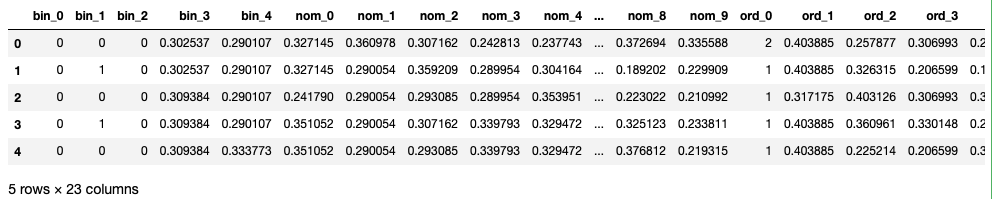
\includegraphics[scale=0.5]{target_sample.png}
            \end{center}
        \end{figure}
    \end{frame}

    \begin{frame}[fragile]
        \frametitle{Leave-one-out Encoder}
        \begin{itemize}
            \item Another target based encoder. Similar to default target encoder with the slight
            difference that to current observation is leave out of calculation.
            \pause
            \item $\hat{x}^k_i = \frac{\sum_{j\neq i} (y_j \cdot (x_j == k))}{\sum_{j\neq i} x_j
                == k}$
            \pause
            \item To prevend the target leakage the formula is augmented by randomness and
            regularization: $\hat{x}^k_i = \frac{\sum_{j\neq i} (y_j \cdot (x_j == k))}{\sum_
                    {j} (x_j== k) - 1 + R} \cdot (1 + \epsilon_i)$
            \item where R is regularization factor and $ \epsilon \approx N(0, \sigma^2)$.
            \pause
            \item Problem is shift in encoding of train and test categories.
            \pause
        \end{itemize}

        \begin{lstlisting}
LOOE_encoder = LeaveOneOutEncoder()
train_looe = LOOE_encoder.fit_transform(train[feature_list], target)
test_looe = LOOE_encoder.transform(test[feature_list])
        \end{lstlisting}
    \end{frame}

    \begin{frame}[fragile]
        \frametitle{M-Estimate Encoder}
        \begin{itemize}
            \item Handles outliers assigning weights to each category based on its deviation from
            overall class frequency.
        \end{itemize}

        \[
            \hat{x}^k = \frac{n^+ + prior \cdot m}{y^+ + m} \m ,
        \] where $m$ is the smoothing hyperparameter.

        \begin{lstlisting}
MEE_encoder = MEstimateEncoder()
train_mee = MEE_encoder.fit_transform(train[feature_list], target)
test_mee = MEE_encoder.transform(test[feature_list])
        \end{lstlisting}
    \end{frame}

    \begin{frame}[fragile]
        \frametitle{Weight of Evidence Encoder}
        \begin{itemize}
            \item Commonly used in credit scoring. It is the measure of "strength" of grouping
            for separating good and bad risk.
            \pause
            \item a = Distribution of Good Credit Outcomes
            \item b = Distribution of Bad Credit Outcomes
            \item WoE = ln(a/b)
            \pause
        \end{itemize}

        In practice, those formulas might lead to target leakage and therefore the WoE is
        calculated with a smoothing hyperparameter.

        \begin{lstlisting}
WOE_encoder = WOEEncoder()
train_woe = WOE_encoder.fit_transform(train[feature_list], target)
test_woe = WOE_encoder.transform(test[feature_list])
        \end{lstlisting}
    \end{frame}

    \begin{frame}[fragile]
        \frametitle{Probability Ratio Encoder}
        \begin{itemize}
            \item Similar to Weight Of Evidence(WoE), with the only difference that the ratio of
            good and bad probability is used.
            \pause
            \item For each label, we calculate the mean of target=1, i.e. the probability of
            being 1 ( P(1) ).
            \pause
            \item Also we calculate the probability of the target=0 ( P(0) ).
            \pause
            \item And then, we calculate the ratio P(1)/P(0) and replace the labels with that ratio.
            \pause
        \end{itemize}

        \begin{lstlisting}
pr_df = df.groupby("month")["target"].mean()
pr_df = pd.DataFrame(pr_df)
pr_df = pr_df.rename(columns = {"target" : "good"})
pr_df["bad"] = 1-pr_df.good
pr_df["bad"] = np.where(pr_df["bad"] == 0, 0.000001, pr_df["bad"])
pr_df["PR"] = pr_df.good / pr_df.bad
df.loc[:, "PR_Encode"] = df["month"].map(pr_df["PR"])
        \end{lstlisting}
    \end{frame}

    \begin{frame}[fragile]
        \frametitle{James-Stein Encoder}
        \begin{itemize}
            \item Estimation of the mean target for category k could be calculated by:
            \pause
            \item $\hat{x}^k = (1-B) \cdot \frac{n^+}{n} + B \cdot \frac{y^+}{y}$
            \pause
        \end{itemize}

        B is a hyperparameter but J-S found a formula to calculate it:
        \[
            B = \frac{Var[y^k]}{Var[y^k] + Var[y]}
        \]

        \pause
        It is defined only for normal distribution. Not the case for any classification task.
        There is workaround for it - using log-odds ratios instead (default option of the
        transformer).
        \begin{lstlisting}
JSE_encoder = JamesSteinEncoder()
train_jse = JSE_encoder.fit_transform(train[feature_list], target)
test_jse = JSE_encoder.transform(test[feature_list])
        \end{lstlisting}
    \end{frame}

    \begin{frame}[fragile]
        \frametitle{Catboost Encoder}
        \begin{itemize}
            \item Catboost is a recently created target-based categorical encoder.
            \pause
            \item Catboost overcomes the target leakage by introducing time into dataset - the
            order of the observations.
            \pause
            \item $\hat{x}^k_i = \frac{\sum_{j = 0}^{j \leq i} (y_j \cdot (x_j == k)) - y_i +
            prior}{\sum_{j = 0}^{j \leq i} (x_j == k) + 1}$
            \pause
            \item To prevent the over-fitting, the process is repeated several times on shuffled
            dataset and results are averaged.
            \pause
            \item Catboost "on-the-fly" encoding is one of the core advantages of CatBoost.
            \pause
        \end{itemize}

        \begin{lstlisting}
CBE_encoder = CatBoostEncoder()
train_cbe = CBE_encoder.fit_transform(train[feature_list], target)
test_cbe = CBE_encoder.transform(test[feature_list])
        \end{lstlisting}
    \end{frame}

    \begin{frame}
        \frametitle{Hashing Encoder}
        \begin{itemize}
            \item Converts categorical variables to a higher dimensional space of integers.
            \pause
            \item Maintains the distance between two vectors of categorical variables
            \pause
            \item The number of dimensions will be far less than One Hot Encoding
            \pause
            \item Data are transformed into fewer features - information loss.
            \pause
            \item Different categorical values could be represented by the same Hash values.
            \pause
            \item Many Kaggle competitors use Hash Encoding to win the competition, so it is
            worth a try.
            \pause
            \item Used in production when a category changes very frequently.
        \end{itemize}
    \end{frame}

    \begin{frame}[fragile]
        \frametitle{Hashing Encoder}
        \begin{lstlisting}
hencoder = HashingEncoder(cols='Temperature',n_components=3)
hash_res = hencoder.fit_transform(df['Temperature'])
hash_res.sample(5)
        \end{lstlisting}
    \end{frame}

    \begin{frame}
        \frametitle{Generalized Linear Mixed Model (GLMM) Encoder }
        \begin{itemize}
            \item Similar to TargetEncoder or M-Estimate Encoder.
            \pause
            \item Solid statistical theory behind the technique.
            \pause
            \item No hyper-parameters to tune. The amount of shrinkage is automatically
            determined through the estimation process.
            \pause
            \item The less observations a category has and/or the more the outcome varies for a
            category then the higher the regularization towards "the prior" or "grand mean".
            \pause
            \item You can just regard this method as applying "GLMM linear regression" on target
            encoding.
            \pause
            \item More time-consuming compare with other methods.
        \end{itemize}
    \end{frame}

    \begin{frame}[fragile]
        \begin{lstlisting}
glmm_encoder = GLMMEncoder(cols=["month"], binomial_target=True)
# binomial_target = True (for Classification)
# binomial_target = False (for Regression)
glmm_encoder.fit(train["month"], target)
X_encoded = glmm_encoder.transform(train["month"])
        \end{lstlisting}
    \end{frame}


    \section{Conclusion}
    \begin{frame}
        \frametitle{Conclusion}
        It is essential to understand that all these encodings do not work well in all situations
        or for every dataset for all machine learning models. Data Scientists still need to
        experiment and find out which works best for their specific case. If test data has
        different classes, some of these methods won't work as features won't be similar. There
        are few benchmark publications by research communities, but it's not conclusive which
        works best.

        My recommendation will be to try each of these with the smaller datasets and
        then decide where to focus on tuning the encoding process.
    \end{frame}
%
%    \begin{frame}
%        \frametitle{Short Guide-Lines}
%        \begin{itemize}
%            \item For \textbf{nominal} columns try \emph{OneHot, Hashing, LeaveOneOut, Target} encoding.
%            \pause
%            \item \textbf{Avoid OneHot for high cardinality columns and decision tree-based algorithms}.
%            \pause
%            \item For \textbf{ordinal} columns try \emph{Ordinal, Binary, OneHot, LeaveOneOut,
%                Target}.
%            \pause
%            \item \emph{Helmert, Sum, BackwardDifference and Polynomial} are less likely to be
%            helpful, but if you have time or theoretic reason you might want to try them.
%            \pause
%            \item For \emph{regression} tasks, Target and LeaveOneOut probably won't work well.
%        \end{itemize}
%    \end{frame}


    \section{XGB with Cross-Validation}
    \begin{frame}
        \frametitle{Cross-Validation}
        \begin{table}[htb]
            \begin{center}
            {\renewcommand{\arraystretch}{0.4}
            \renewcommand{\tabcolsep}{0.4cm}
                \begin{tabular}[c]{|c|c|c|c|}
                    \hline
                    \textbf{Label}     & \textbf{train} & \textbf{val} & \textbf{test} \\
                    \hline
                    OrdinalEncoder     & 0.85611        & 0.76588      & 0.76459       \\
                    \hline
                    WOEEncoder         & 0.86433        & 0.83322      & 0.77296       \\
                    \hline
                    TargetEncoder      & 0.86220        & 0.82985      & 0.77866       \\
                    \hline
                    MEstimateEncoder   & 0.86547        & 0.83427      & 0.77057       \\
                    \hline
                    JamesSteinEncoder  & 0.86547        & 0.83469      & 0.76749       \\
                    \hline
                    LeaveOneOutEncoder & 1.00000        & 1.00000      & 0.51884       \\
                    \hline
                    CatBoostEncoder    & 0.82644        & 0.78127      & 0.78850       \\
                    \hline
                    HashingEncoder     & 0.63969        & 0.62233      & 0.61618       \\
                    \hline
                    OneHotEncoder      & 0.85759        & 0.77439      & 0.77330       \\
                    \hline
                \end{tabular}}
                \caption{XGB CV}
            \end{center}
        \end{table}
    \end{frame}


    \section{End of Story}
    \begin{frame}
        \frametitle{The End}
        Thank you for your attention and patience.
    \end{frame}


\end{document}
